\documentclass{techbrief}

\usepackage{tikz}
\usetikzlibrary{shapes.geometric, calc}

\title{Relationship between formulations of classical mechanics}
\author{Gabriele Carcassi}
\category{Classical mechanics}
\tags{Newtonian mechanics, Lagrangian mechanics, Hamiltonian mechanics}

\begin{document}
	
	\maketitle
	
	\begin{abstract}
		We show that the three formulations in classical mechanics are not equivalent and the relationship between them. We find Newtonian and Hamiltonian mechanics to be independent while Lagrangian mechanics is their intersection.

	\end{abstract}
	
	\section{Introduction}
	While it is often stated that the three formulations in classical mechanics, Newtonian, Lagrangian, and Hamiltonian, are equivalent, there are systems that can be described in one formulation but not another. In this note, we show Newtonian and Hamiltonian mechanics are independent and Lagrangian mechanics is the intersection of the other two.
	\section{Conditions}
		\begin{condition}[Newtonian Mechanics]{NM}
			The state of the system is described by position $x^{i}$ and velocity $v^{i}$. The dynamics is specified by forces $F^{i}(x^{j},v^{k},t)$ which are locally Lipschitz continuous. The evolution of the system over time $t$ is given by the equations $F^{i} = d_{t}(mv^{i})$ where $m$ is the mass of the system.
		\end{condition}
		
		\begin{condition}[Hamiltonian Mechanics]{HM}
			The state of the system is described by position $q^{i}$ and conjugate momentum $p_{i}$. The dynamics is specified by a Hamiltonian $H(q^{i},p_{j},t)$ which is differentiable and whose derivatives are must be at least Lipschitz continuous. The evolution of the system over time $t$ is given by the equations $d_{t}q^{i} = \partial_{p_{i}}H$ and $d_{t}p_{i} = -\partial_{q^{i}}H$.
		\end{condition}
		
		\begin{condition}[Lagrangian Mechanics]{LM}
			The state of the system is described by position $x^{i}$ and velocity $v^{i}$. The dynamics is specified by a Lagrangian $L(x^{i},v^{j},t)$ with the property that the Hessian matrix $\partial_{v^{i}}\partial_{v^{j}}L$ is invertible. The evolution of the system over time $t$ is given by the equations $\partial_{x^{i}}L = d_{t}\partial_{v^{i}}L$.
		\end{condition}
	
	\section{Theorems}
	\begin{thrm}
		Condition \ref{LM} is equivalent to \ref{NM} and \ref{HM}.
	\end{thrm}
	\begin{proof}
		We first show that \ref{LM} implies \ref{NM}. Given a fixed mass and frame, we can find we can explicitly map a unique evolution for \ref{NM}, $d_{t}v^{i}$ or $a^{i}$, given the evolution of the system in \ref{LM}:
		\begin{equation}
			\begin{aligned}
				\partial_{x^i}L&= d_t \partial_{v^i} L \\ &= \partial_{x^j} \partial_{v^i} L d_t x^j + \partial_{v^k} \partial_{v^i} L \, d_t v^k \\ &= \partial_{x^j} \partial_{v^i} L \, v^j + \partial_{v^k} \partial_{v^i} L \, a^k \\
				\partial_{v^k} \partial_{v^i} L \, a^k &= \partial_{x^i}L - \partial_{x^j} \partial_{v^i} L \, v^j .
			\end{aligned}
		\end{equation} 
		Note that we assumed the Hessian matrix $\partial_{v^{i}}\partial_{v^{j}}L$ is invertible, therefore the acceleration can be written explicitly. \\
		
		We can then show that \ref{LM} implies \ref{HM}. We can equate the states through
		\begin{equation}
			\begin{aligned}
				x^{i} &= q^{i} \\
				v^{i} = d_{t}q^{i} &= \partial_{p_{i}}H \\
				p_{i} &= \partial_{v^{i}}L
			\end{aligned}
		\end{equation}
		Then we can find the Hamiltonian from the Lagrangian:
		\begin{equation}
			\left| \partial_{v^i} \partial_{v^j} L \right| = \left| \partial_{v^i} p_j \right| = \left| \partial_{p_i} v^j \right|^{-1} = \left|\partial_{p_i}\partial_{p_j} H\right|^{-1}
		\end{equation}
		Again, $\partial_{v^{i}}\partial_{v^{j}}L$ is invertible so this will always yield a result. \\
		
		We have shown \ref{LM} implies both \ref{NM} and \ref{HM}, and therefore its equivalence.
	\end{proof}
	\begin{thrm}
		Conditions \ref{NM} and \ref{HM} are independent
	\end{thrm}
	\begin{proof}
	We first show that \ref{NM} does not imply \ref{HM}. The dynamics in \ref{NM} requires multiple independently chosen forces whereas in \ref{HM} is specified by a single function, the Hamiltonian. A continuous surjective map from the space of a single function to multiple functions does not exist, therefore there exist systems that can be described by \ref{NM} that cannot be described by \ref{HM}. \\

	We now show that \ref{HM} does not imply \ref{NM} with an example. When treating the photon as a classical particle, we write the Hamiltonian by expressing the energy as a function of momentum
	\begin{equation}
		H=\hbar | \omega| = c \hbar |k| = c |p|.
	\end{equation}
	We can then find to evolution of the particle to be
	\begin{equation}
		\begin{aligned}
			d_t q^i &= c \frac{p^i}{|p|} \\
			d_t p_i &= 0.
		\end{aligned}
	\end{equation} 
	The velocity of the photon is fixed as $c$ while the momentum remains unconstrained. Therefore, there is no way to map the state variables from \ref{HM} to \ref{NM} as the momentum cannot be reconstructed from the velocity.
	
	We have shown that there exist \ref{NM} systems that cannot be expressed with \ref{HM} and vice versa, therefore \ref{NM} and \ref{HM} are independent.
	\end{proof}
	
	Note that by both Theorem 1 and Theorem 5 we can see that neither \ref{NM} or \ref{HM} imply \ref{LM} in isolation.
	
	\begin{figure}[h]
		\centering
		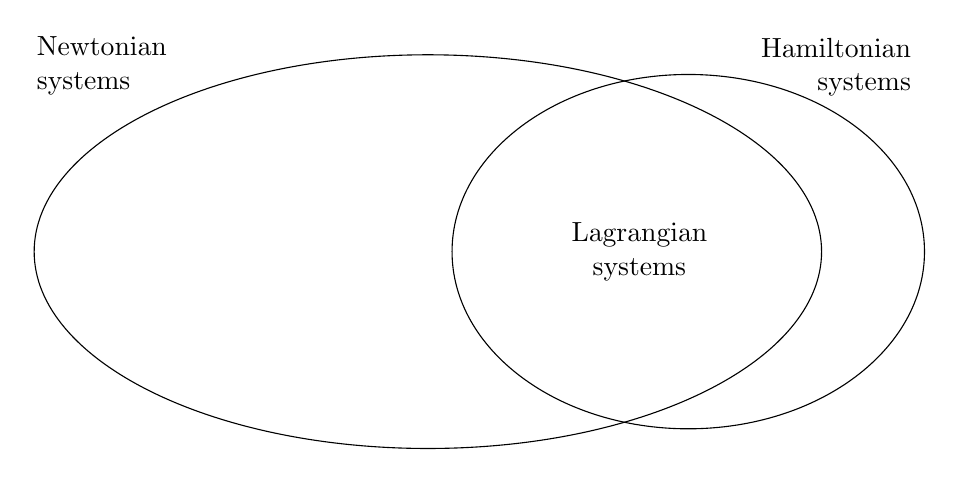
\begin{tikzpicture}
			\node[ellipse, minimum width=10cm, minimum height=5cm, draw, left] (ns){};
			\node [align=left, above] at ([xshift=-6mm,yshift=1mm]ns.north west) {Newtonian \\systems};
			
			\node[ellipse, minimum width=6cm, minimum height=4.5cm, draw] (hs) at ([xshift=-1.7cm]ns.east){};
			\node [align=right, above right] at ([xshift=8mm, yshift=-4mm]hs.north) {Hamiltonian\\ systems};
			\node [align=center, right] at ([xshift=14
			mm]hs.west) {Lagrangian \\systems};
		\end{tikzpicture}
		\caption {Not all Hamiltonian systems are Newtonian and not all Newtonian systems are Hamiltonian. All Lagrangian systems are both Newtonian and Hamiltonian.}\label{rp-cm-fig-vennDiagramEarly}
	\end{figure}
	\section{Conclusion}
		We have found a more precise relationship between the three formulations in classical mechanics. It would be ideal that these distinctions were clarified in introductory physics courses.
	
	
\end{document}